%%%%%%%%%%%%%%%%%%%%%%%%%%%%%%%%%
% PACKAGE IMPORTS
%%%%%%%%%%%%%%%%%%%%%%%%%%%%%%%%%

\def\checkmark{\tikz\fill[scale=0.4](0,.35) -- (.25,0) -- (1,.7) -- (.25,.15) -- cycle;} 
\usepackage[tmargin=2cm,rmargin=1in,lmargin=1in,margin=0.85in,bmargin=2cm,footskip=.2in]{geometry}
\usepackage{amsmath,amsfonts,amsthm,amssymb,mathtools}
% \usepackage[varbb]{newpxmath}
\usepackage{lipsum} % for generating dummy text
% \usepackage{fontawesome} % for icons
\usepackage{fontawesome5} % for icons
\usepackage{titlesec}
\usepackage{xfrac}
\usepackage{changepage}
\usepackage{geometry}
\usepackage[makeroom]{cancel}
\usepackage{mathtools}
\usepackage{esdiff}
\usepackage{bookmark}
\usepackage{enumitem}
\usepackage{hyperref,theoremref}
\usepackage[]{mdframed}
\usepackage{pgfpages}
\usepackage{pgfplots}
\pgfplotsset{compat=1.18} % Add this line to set the compatibility version
\usepackage{pgfmath}
\usepackage{fancyhdr}
\usepackage{pifont}
\usepackage{tocloft}
\setcounter{tocdepth}{3}
\setcounter{secnumdepth}{3}
\usepackage{multirow}
\usepackage{dcolumn}
\usepackage{tikz}
\usepackage{minted}
% \usepackage{listings}
\usepackage[bottom]{footmisc}
\newcolumntype{2}{D{.}{}{2.0}}
\newcommand{\summation}[2]{\sum\limits^{#1}_{#2}}
\hypersetup{
	pdftitle={Assignment},
	colorlinks=true,
	linkcolor=black,
	bookmarksnumbered=true,
	bookmarksopen=true
}
\usepackage[most,many,breakable]{tcolorbox}
\usepackage{xcolor}
\usepackage{varwidth}
\usepackage{varwidth}
\usepackage{etoolbox}
%\usepackage{authblk}
\usepackage{nameref}
\usepackage{multicol,array}
\usepackage{tikz-cd}
\usepackage[ruled,vlined,linesnumbered]{algorithm2e}
\usepackage{comment} % enables the use of multi-line comments (\ifx \fi) 
\usepackage{import}
\usepackage{xifthen}
\usepackage{pdfpages}
\usepackage{transparent}
\usepackage{longtable}
\usepackage{graphicx}
% \usepackage{table}

% NAND and NOR define
\makeatletter
\DeclareRobustCommand{\nand}{\mathbin{\mathpalette\n@and@or\land}}
\DeclareRobustCommand{\nor}{\mathbin{\mathpalette\n@and@or\lor}}

\newcommand{\n@and@or}[2]{%
  	\vphantom{#2}%
  	\ooalign{$\m@th#1#2$\cr\hidewidth$\m@th#1\sim$\hidewidth\cr}%
}
\makeatother

% Start sections at 1
\renewcommand{\thesection}{\arabic{section}}
\renewcommand{\thesubsection}{\thesection.\arabic{subsection}}
\renewcommand{\thesubsubsection}{\thesubsection.\arabic{subsubsection}}

\newcommand\mycommfont[1]{\footnotesize\ttfamily\textcolor{blue}{#1}}
\SetCommentSty{mycommfont}
\newcommand{\incfig}[1]{%
    % \def\svgwidth{\columnwidth}
    % \def\svgwidth{\textwidth}
    \import{./figures/}{#1.pdf_tex}
}

\usepackage{tikzsymbols}
\renewcommand\qedsymbol{$\Laughey$}

\newcommand*\Heq{\ensuremath{\overset{\kern2pt H}{=}}}

\renewcommand{\mathsection}[2]{
  	\pagebreak \bigbreak \noindent
  	\begin{Large}
      	\begin{mdframed}
          	\begin{center}
              	\textbf{#1}
          	\end{center}
      	\end{mdframed}
  	\end{Large}
  	\begin{Large}
      	\begin{center}
          	\textbf{#2}
      	\end{center}
  	\end{Large}
  	\line(1,0){490}
}

% Custom Theorem Box
\newtcbtheorem[number within=section]{theo}{Theorem.}%
{colback=white!5,colframe=black!35!black,fonttitle=\bfseries}{th}

\usepackage{import}
\usepackage{xifthen}
\usepackage{pdfpages}
\usepackage{transparent}


%%%%%%%%%%%%%%%%%%%%%%%%%%%%%%
% SELF MADE COLORS
%%%%%%%%%%%%%%%%%%%%%%%%%%%%%%



\definecolor{myg}{RGB}{56, 140, 70}
\definecolor{myb}{RGB}{45, 111, 177}
\definecolor{myr}{RGB}{199, 68, 64}
\definecolor{mytheorembg}{HTML}{F2F2F9}
\definecolor{mytheoremfr}{HTML}{00007B}
\definecolor{mylenmabg}{HTML}{FFFAF8}
\definecolor{mylenmafr}{HTML}{983b0f}
\definecolor{mypropbg}{HTML}{f2fbfc}
\definecolor{mypropfr}{HTML}{191971}
\definecolor{myexamplebg}{HTML}{F2FBF8}
\definecolor{myexamplefr}{HTML}{88D6D1}
\definecolor{myexampleti}{HTML}{2A7F7F}
\definecolor{mydefinitbg}{HTML}{E5E5FF}
\definecolor{mydefinitfr}{HTML}{3F3FA3}
\definecolor{notesgreen}{RGB}{0,162,0}
\definecolor{myp}{RGB}{197, 92, 212}
\definecolor{mygr}{HTML}{2C3338}
\definecolor{myred}{RGB}{127,0,0}
\definecolor{myyellow}{RGB}{169,121,69}
\definecolor{myexercisebg}{HTML}{F2FBF8}
\definecolor{myexercisefg}{HTML}{88D6D1}


%%%%%%%%%%%%%%%%%%%%%%%%%%%%
% TCOLORBOX SETUPS
%%%%%%%%%%%%%%%%%%%%%%%%%%%%

\setlength{\parindent}{1cm}
%================================
% THEOREM BOX
%================================

\tcbuselibrary{theorems,skins,hooks}
\newtcbtheorem[number within=section]{Theorem}{Theorem}
{%
	enhanced,
	breakable,
	colback = mytheorembg,
	frame hidden,
	boxrule = 0sp,
	borderline west = {2pt}{0pt}{mytheoremfr},
	sharp corners,
	detach title,
	before upper = \tcbtitle\par\smallskip,
	coltitle = mytheoremfr,
	fonttitle = \bfseries\sffamily,
	description font = \mdseries,
	separator sign none,
	segmentation style={solid, mytheoremfr},
}
{th}

\tcbuselibrary{theorems,skins,hooks}
\newtcbtheorem[number within=chapter]{theorem}{Theorem}
{%
	enhanced,
	breakable,
	colback = mytheorembg,
	frame hidden,
	boxrule = 0sp,
	borderline west = {2pt}{0pt}{mytheoremfr},
	sharp corners,
	detach title,
	before upper = \tcbtitle\par\smallskip,
	coltitle = mytheoremfr,
	fonttitle = \bfseries\sffamily,
	description font = \mdseries,
	separator sign none,
	segmentation style={solid, mytheoremfr},
}
{th}


\tcbuselibrary{theorems,skins,hooks}
\newtcolorbox{Theoremcon}
{%
	enhanced
	,breakable
	,colback = mytheorembg
	,frame hidden
	,boxrule = 0sp
	,borderline west = {2pt}{0pt}{mytheoremfr}
	,sharp corners
	,description font = \mdseries
	,separator sign none
}
%
% %================================
% % Corollery
% %================================
% \tcbuselibrary{theorems,skins,hooks}
% \newtcbtheorem[number within=section]{Corollary}{Corollary}
% {%
% 	enhanced
% 	,breakable
% 	,colback = myp!10
% 	,frame hidden
% 	,boxrule = 0sp
% 	,borderline west = {2pt}{0pt}{myp!85!black}
% 	,sharp corners
% 	,detach title
% 	,before upper = \tcbtitle\par\smallskip
% 	,coltitle = myp!85!black
% 	,fonttitle = \bfseries\sffamily
% 	,description font = \mdseries
% 	,separator sign none
% 	,segmentation style={solid, myp!85!black}
% }
% {th}
% \tcbuselibrary{theorems,skins,hooks}
% \newtcbtheorem[number within=chapter]{corollary}{Corollary}
% {%
% 	enhanced
% 	,breakable
% 	,colback = myp!10
% 	,frame hidden
% 	,boxrule = 0sp
% 	,borderline west = {2pt}{0pt}{myp!85!black}
% 	,sharp corners
% 	,detach title
% 	,before upper = \tcbtitle\par\smallskip
% 	,coltitle = myp!85!black
% 	,fonttitle = \bfseries\sffamily
% 	,description font = \mdseries
% 	,separator sign none
% 	,segmentation style={solid, myp!85!black}
% }
% {th}
%
%
% %================================
% % LENMA
% %================================
%
% \tcbuselibrary{theorems,skins,hooks}
% \newtcbtheorem[number within=section]{Lenma}{Lenma}
% {%
% 	enhanced,
% 	breakable,
% 	colback = mylenmabg,
% 	frame hidden,
% 	boxrule = 0sp,
% 	borderline west = {2pt}{0pt}{mylenmafr},
% 	sharp corners,
% 	detach title,
% 	before upper = \tcbtitle\par\smallskip,
% 	coltitle = mylenmafr,
% 	fonttitle = \bfseries\sffamily,
% 	description font = \mdseries,
% 	separator sign none,
% 	segmentation style={solid, mylenmafr},
% }
% {th}
%
% \tcbuselibrary{theorems,skins,hooks}
% \newtcbtheorem[number within=chapter]{lenma}{Lenma}
% {%
% 	enhanced,
% 	breakable,
% 	colback = mylenmabg,
% 	frame hidden,
% 	boxrule = 0sp,
% 	borderline west = {2pt}{0pt}{mylenmafr},
% 	sharp corners,
% 	detach title,
% 	before upper = \tcbtitle\par\smallskip,
% 	coltitle = mylenmafr,
% 	fonttitle = \bfseries\sffamily,
% 	description font = \mdseries,
% 	separator sign none,
% 	segmentation style={solid, mylenmafr},
% }
% {th}
%
%
% %================================
% % PROPOSITION
% %================================
%
% \tcbuselibrary{theorems,skins,hooks}
% \newtcbtheorem[number within=section]{Prop}{Proposition}
% {%
% 	enhanced,
% 	breakable,
% 	colback = mypropbg,
% 	frame hidden,
% 	boxrule = 0sp,
% 	borderline west = {2pt}{0pt}{mypropfr},
% 	sharp corners,
% 	detach title,
% 	before upper = \tcbtitle\par\smallskip,
% 	coltitle = mypropfr,
% 	fonttitle = \bfseries\sffamily,
% 	description font = \mdseries,
% 	separator sign none,
% 	segmentation style={solid, mypropfr},
% }
% {th}
%
% \tcbuselibrary{theorems,skins,hooks}
% \newtcbtheorem[number within=chapter]{prop}{Proposition}
% {%
% 	enhanced,
% 	breakable,
% 	colback = mypropbg,
% 	frame hidden,
% 	boxrule = 0sp,
% 	borderline west = {2pt}{0pt}{mypropfr},
% 	sharp corners,
% 	detach title,
% 	before upper = \tcbtitle\par\smallskip,
% 	coltitle = mypropfr,
% 	fonttitle = \bfseries\sffamily,
% 	description font = \mdseries,
% 	separator sign none,
% 	segmentation style={solid, mypropfr},
% }
% {th}
%

%================================
% CLAIM
%================================

\tcbuselibrary{theorems,skins,hooks}
\newtcbtheorem[number within=section]{claim}{Claim}
{%
	enhanced
	,breakable
	,colback = myg!10
	,frame hidden
	,boxrule = 0sp
	,borderline west = {2pt}{0pt}{myg}
	,sharp corners
	,detach title
	,before upper = \tcbtitle\par\smallskip
	,coltitle = myg!85!black
	,fonttitle = \bfseries\sffamily
	,description font = \mdseries
	,separator sign none
	,segmentation style={solid, myg!85!black}
}
{th}



%================================
% Exercise
%================================

\tcbuselibrary{theorems,skins,hooks}
\newtcbtheorem[number within=section]{Exercise}{Exercise}
{%
	enhanced,
	breakable,
	colback = myexercisebg,
	frame hidden,
	boxrule = 0sp,
	borderline west = {2pt}{0pt}{myexercisefg},
	sharp corners,
	detach title,
	before upper = \tcbtitle\par\smallskip,
	coltitle = myexercisefg,
	fonttitle = \bfseries\sffamily,
	description font = \mdseries,
	separator sign none,
	segmentation style={solid, myexercisefg},
}
{th}

\tcbuselibrary{theorems,skins,hooks}
\newtcbtheorem[number within=chapter]{exercise}{Exercise}
{%
	enhanced,
	breakable,
	colback = myexercisebg,
	frame hidden,
	boxrule = 0sp,
	borderline west = {2pt}{0pt}{myexercisefg},
	sharp corners,
	detach title,
	before upper = \tcbtitle\par\smallskip,
	coltitle = myexercisefg,
	fonttitle = \bfseries\sffamily,
	description font = \mdseries,
	separator sign none,
	segmentation style={solid, myexercisefg},
}
{th}

%================================
% EXAMPLE BOX
%================================

\newtcbtheorem[number within=section]{Example}{Example}
{%
	colback = myexamplebg
	,breakable
	,colframe = myexamplefr
	,coltitle = myexampleti
	,boxrule = 1pt
	,sharp corners
	,detach title
	,before upper=\tcbtitle\par\smallskip
	,fonttitle = \bfseries
	,description font = \mdseries
	,separator sign none
	,description delimiters parenthesis
}
{ex}

\newtcbtheorem[number within=chapter]{example}{Example}
{%
	colback = myexamplebg
	,breakable
	,colframe = myexamplefr
	,coltitle = myexampleti
	,boxrule = 1pt
	,sharp corners
	,detach title
	,before upper=\tcbtitle\par\smallskip
	,fonttitle = \bfseries
	,description font = \mdseries
	,separator sign none
	,description delimiters parenthesis
}
{ex}

%================================
% DEFINITION BOX
%================================
%
% \newtcbtheorem[number within=section]{Definition}{Definition}{enhanced,
% 	before skip=2mm,after skip=2mm, colback=red!5,colframe=red!80!black,boxrule=0.5mm,
% 	attach boxed title to top left={xshift=1cm,yshift*=1mm-\tcboxedtitleheight}, varwidth boxed title*=-3cm,
% 	boxed title style={frame code={
% 					\path[fill=tcbcolback]
% 					([yshift=-1mm,xshift=-1mm]frame.north west)
% 					arc[start angle=0,end angle=180,radius=1mm]
% 					([yshift=-1mm,xshift=1mm]frame.north east)
% 					arc[start angle=180,end angle=0,radius=1mm];
% 					\path[left color=tcbcolback!60!black,right color=tcbcolback!60!black,
% 						middle color=tcbcolback!80!black]
% 					([xshift=-2mm]frame.north west) -- ([xshift=2mm]frame.north east)
% 					[rounded corners=1mm]-- ([xshift=1mm,yshift=-1mm]frame.north east)
% 					-- (frame.south east) -- (frame.south west)
% 					-- ([xshift=-1mm,yshift=-1mm]frame.north west)
% 					[sharp corners]-- cycle;
% 				},interior engine=empty,
% 		},
% 	fonttitle=\bfseries,
% 	title={#2},#1}{def}
% \newtcbtheorem[number within=chapter]{definition}{Definition}{enhanced,
% 	before skip=2mm,after skip=2mm, colback=red!5,colframe=red!80!black,boxrule=0.5mm,
% 	attach boxed title to top left={xshift=1cm,yshift*=1mm-\tcboxedtitleheight}, varwidth boxed title*=-3cm,
% 	boxed title style={frame code={
% 					\path[fill=tcbcolback]
% 					([yshift=-1mm,xshift=-1mm]frame.north west)
% 					arc[start angle=0,end angle=180,radius=1mm]
% 					([yshift=-1mm,xshift=1mm]frame.north east)
% 					arc[start angle=180,end angle=0,radius=1mm];
% 					\path[left color=tcbcolback!60!black,right color=tcbcolback!60!black,
% 						middle color=tcbcolback!80!black]
% 					([xshift=-2mm]frame.north west) -- ([xshift=2mm]frame.north east)
% 					[rounded corners=1mm]-- ([xshift=1mm,yshift=-1mm]frame.north east)
% 					-- (frame.south east) -- (frame.south west)
% 					-- ([xshift=-1mm,yshift=-1mm]frame.north west)
% 					[sharp corners]-- cycle;
% 				},interior engine=empty,
% 		},
% 	fonttitle=\bfseries,
% 	title={#2},#1}{def}
%
%

%================================
% Solution BOX
%================================

\makeatletter
\newtcbtheorem{question}{Question}{enhanced,
	breakable,
	colback=white,
	colframe=myb!80!black,
	attach boxed title to top left={yshift*=-\tcboxedtitleheight},
	fonttitle=\bfseries,
	title={#2},
	boxed title size=title,
	boxed title style={%
		sharp corners,
		rounded corners=northwest,
		colback=tcbcolframe,
		boxrule=0pt,
	},
	underlay boxed title={%
		\path[fill=tcbcolframe] (title.south west)--(title.south east)
		to[out=0, in=180] ([xshift=5mm]title.east)--
		(title.center-|frame.east)
		[rounded corners=\kvtcb@arc] |-
		(frame.north) -| cycle;
	},
	#1
}{def}
\makeatother

%================================
% SOLUTION BOX
%================================

\makeatletter
\newtcolorbox{solution}{enhanced,
	breakable,
	colback=white,
	colframe=myg!80!black,
	attach boxed title to top left={yshift*=-\tcboxedtitleheight},
	title=Solution,
	boxed title size=title,
	boxed title style={%
		sharp corners,
		rounded corners=northwest,
		colback=tcbcolframe,
		boxrule=0pt,
	},
	underlay boxed title={%
		\path[fill=tcbcolframe] (title.south west)--(title.south east)
		to[out=0, in=180] ([xshift=5mm]title.east)--
		(title.center-|frame.east)
		[rounded corners=\kvtcb@arc] |-
		(frame.north) -| cycle;
	},
}
\makeatother

%================================
% Question BOX
%================================

\makeatletter
\newtcbtheorem{qstion}{Question}{enhanced,
	breakable,
	colback=white,
	colframe=mygr,
	attach boxed title to top left={yshift*=-\tcboxedtitleheight},
	fonttitle=\bfseries,
	title={#2},
	boxed title size=title,
	boxed title style={%
		sharp corners,
		rounded corners=northwest,
		colback=tcbcolframe,
		boxrule=0pt,
	},
	underlay boxed title={%
		\path[fill=tcbcolframe] (title.south west)--(title.south east)
		to[out=0, in=180] ([xshift=5mm]title.east)--
		(title.center-|frame.east)
		[rounded corners=\kvtcb@arc] |-
		(frame.north) -| cycle;
	},
	#1
}{def}
\makeatother

\newtcbtheorem[number within=chapter]{wconc}{Wrong Concept}{
	breakable,
	enhanced,
	colback=white,
	colframe=myr,
	arc=0pt,
	outer arc=0pt,
	fonttitle=\bfseries\sffamily\large,
	colbacktitle=myr,
	attach boxed title to top left={},
	boxed title style={
		enhanced,
		skin=enhancedfirst jigsaw,
		arc=3pt,
		bottom=0pt,
		interior style={fill=myr}
	},
	#1
}{def}



%================================
% NOTE BOX
%================================

\usetikzlibrary{arrows,calc,shadows.blur}
\tcbuselibrary{skins}
\newtcolorbox{note}[1][]{%
	enhanced jigsaw,
	colback=white!20!white,%
	colframe=black!80!white,
	% size=small,
	boxrule=1pt,
	title=\textbf{Note:-},
	halign title=flush center,
	coltitle=black,
	breakable,
	drop shadow=black!50!white,
	attach boxed title to top left={xshift=1cm,yshift=-\tcboxedtitleheight/2,yshifttext=-\tcboxedtitleheight/2},
	minipage boxed title=1.5cm,
	boxed title style={%
		colback=white,
		size=fbox,
		boxrule=1pt,
		boxsep=2pt,
		underlay={%
			\coordinate (dotA) at ($(interior.west) + (-0.5pt,0)$);
			\coordinate (dotB) at ($(interior.east) + (0.5pt,0)$);
			\begin{scope}
				\clip (interior.north west) rectangle ([xshift=3ex]interior.east);
				\filldraw [white, blur shadow={shadow opacity=60, shadow yshift=-.75ex}, rounded corners=2pt] (interior.north west) rectangle (interior.south east);
			\end{scope}
			\begin{scope}[gray!80!black]
				\fill (dotA) circle (2pt);
				\fill (dotB) circle (2pt);
			\end{scope}
		},
	},
	#1,
}

% %================================
% % Theorem BOX
% %================================
\newtcolorbox[auto counter]{thrm}[1][\empty]{%
	enhanced jigsaw,
	colback=white!20!white,%
	colframe=blue!80!blue,
	boxrule=1.25pt,
	title=\textbf{Theorem \thetcbcounter\ifx#1\empty\else: #1\fi},
	halign title=flush center,
	coltitle=black,
	breakable,
	drop shadow=black!50!white,
	attach boxed title to top left={xshift=1cm,yshift=-\tcboxedtitleheight/2,yshifttext=-\tcboxedtitleheight/2},
	% Uncomment to statically determine length of title box, otherwise keep it dynamic
	% minipage boxed title=3cm,
	boxed title style={%
		colback=white,
		size=fbox,
		boxrule=1pt,
		boxsep=2pt,
		underlay={%
			\coordinate (dotA) at ($(interior.west) + (-0.5pt,0)$);
			\coordinate (dotB) at ($(interior.east) + (0.5pt,0)$);
			\begin{scope}
				\clip (interior.north west) rectangle ([xshift=3ex]interior.east);
				\filldraw [white, blur shadow={shadow opacity=60, shadow yshift=-.75ex}, rounded corners=2pt] (interior.north west) rectangle (interior.south east);
			\end{scope}
			\begin{scope}[gray!80!black]
				\fill (dotA) circle (2pt);
				\fill (dotB) circle (2pt);
			\end{scope}
		},
	},
}
%
% % \usepackage{etoolbox}
% % \preto{\section}{\setcounter{tcbcounter}{0}}
% \usetikzlibrary{arrows,calc,shadows.blur}
% \tcbuselibrary{skins}
% \newtcolorbox[auto counter]{thrm}[1][]{%
% 	enhanced jigsaw,
% 	colback=white!20!white,%
% 	colframe=blue!80!blue,
% 	boxrule=1.25pt,
% 	title=\textbf{Theorem \thetcbcounter:},
% 	halign title=flush center,
% 	coltitle=black,
% 	breakable,
% 	drop shadow=black!50!white,
% 	attach boxed title to top left={xshift=1cm,yshift=-\tcboxedtitleheight/2,yshifttext=-\tcboxedtitleheight/2},
% 	minipage boxed title=2.5cm,
% 	boxed title style={%
% 		colback=white,
% 		size=fbox,
% 		boxrule=1pt,
% 		boxsep=2pt,
% 		underlay={%
% 			\coordinate (dotA) at ($(interior.west) + (-0.5pt,0)$);
% 			\coordinate (dotB) at ($(interior.east) + (0.5pt,0)$);
% 			\begin{scope}
% 				\clip (interior.north west) rectangle ([xshift=3ex]interior.east);
% 				\filldraw [white, blur shadow={shadow opacity=60, shadow yshift=-.75ex}, rounded corners=2pt] (interior.north west) rectangle (interior.south east);
% 			\end{scope}
% 			\begin{scope}[gray!80!black]
% 				\fill (dotA) circle (2pt);
% 				\fill (dotB) circle (2pt);
% 			\end{scope}
% 		},
% 	},
% 	#1,
% }
%
%================================
% Definition BOX
%================================

% \usepackage{etoolbox}
% \preto{\section}{\setcounter{tcbcounter}{0}}
\usetikzlibrary{arrows,calc,shadows.blur}
\tcbuselibrary{skins}
\newtcolorbox[auto counter]{definition}[1][]{%
	enhanced jigsaw,
	colback=white!20!white,%
	colframe=green!80!green,
	boxrule=1.25pt,
	title=\textbf{Definition \thetcbcounter:},
	halign title=flush center,
	coltitle=black,
	breakable,
	drop shadow=black!50!white,
	attach boxed title to top left={xshift=1cm,yshift=-\tcboxedtitleheight/2,yshifttext=-\tcboxedtitleheight/2},
	minipage boxed title=2.5cm,
	boxed title style={%
		colback=white,
		size=fbox,
		boxrule=1pt,
		boxsep=2pt,
		underlay={%
			\coordinate (dotA) at ($(interior.west) + (-0.5pt,0)$);
			\coordinate (dotB) at ($(interior.east) + (0.5pt,0)$);
			\begin{scope}
				\clip (interior.north west) rectangle ([xshift=3ex]interior.east);
				\filldraw [white, blur shadow={shadow opacity=60, shadow yshift=-.75ex}, rounded corners=2pt] (interior.north west) rectangle (interior.south east);
			\end{scope}
			\begin{scope}[gray!80!black]
				\fill (dotA) circle (2pt);
				\fill (dotB) circle (2pt);
			\end{scope}
		},
	},
	#1,
}

%================================
% Example BOX
%================================

\newtcolorbox[auto counter]{eg}[1][\empty]{%
	enhanced jigsaw,
	colback=white!20!white,%
	colframe=red!80!red,
	boxrule=1.25pt,
	title=\textbf{Example \thetcbcounter\ifx#1\empty\else: #1\fi},
	halign title=flush center,
	coltitle=black,
	breakable,
	drop shadow=black!50!white,
	attach boxed title to top left={xshift=1cm,yshift=-\tcboxedtitleheight/2,yshifttext=-\tcboxedtitleheight/2},
	% Uncomment to statically determine length of title box, otherwise keep it dynamic
	% minipage boxed title=3cm,
	boxed title style={%
		colback=white,
		size=fbox,
		boxrule=1pt,
		boxsep=2pt,
		underlay={%
			\coordinate (dotA) at ($(interior.west) + (-0.5pt,0)$);
			\coordinate (dotB) at ($(interior.east) + (0.5pt,0)$);
			\begin{scope}
				\clip (interior.north west) rectangle ([xshift=3ex]interior.east);
				\filldraw [white, blur shadow={shadow opacity=60, shadow yshift=-.75ex}, rounded corners=2pt] (interior.north west) rectangle (interior.south east);
			\end{scope}
			\begin{scope}[gray!80!black]
				\fill (dotA) circle (2pt);
				\fill (dotB) circle (2pt);
			\end{scope}
		},
	},
}
%
% % \usepackage{etoolbox}
% % \preto{\section}{\setcounter{tcbcounter}{0}}
% \usetikzlibrary{arrows,calc,shadows.blur}
% \tcbuselibrary{skins}
% \newtcolorbox[auto counter]{eg}[1][]{%
% 	enhanced jigsaw,
% 	colback=white!20!white,%
% 	colframe=red!80!red,
% 	boxrule=1.25pt,
% 	title=\textbf{Example \thetcbcounter:},
% 	halign title=flush center,
% 	coltitle=black,
% 	breakable,
% 	drop shadow=black!50!white,
% 	attach boxed title to top left={xshift=1cm,yshift=-\tcboxedtitleheight/2,yshifttext=-\tcboxedtitleheight/2},
% 	minipage boxed title=2.5cm,
% 	boxed title style={%
% 		colback=white,
% 		size=fbox,
% 		boxrule=1pt,
% 		boxsep=2pt,
% 		underlay={%
% 			\coordinate (dotA) at ($(interior.west) + (-0.5pt,0)$);
% 			\coordinate (dotB) at ($(interior.east) + (0.5pt,0)$);
% 			\begin{scope}
% 				\clip (interior.north west) rectangle ([xshift=3ex]interior.east);
% 				\filldraw [white, blur shadow={shadow opacity=60, shadow yshift=-.75ex}, rounded corners=2pt] (interior.north west) rectangle (interior.south east);
% 			\end{scope}
% 			\begin{scope}[gray!80!black]
% 				\fill (dotA) circle (2pt);
% 				\fill (dotB) circle (2pt);
% 			\end{scope}
% 		},
% 	},
% 	#1,
% }
%
%
%
\usepackage{mdframed}
\mdfsetup{skipabove=1em,skipbelow=0em}
\theoremstyle{definition}
% \newmdtheoremenv[nobreak=true]{definition}{Definition}
% \newmdtheoremenv[nobreak=true]{property}{Property}
\newmdtheoremenv[nobreak=true]{consequence}{Consequence}
% \newmdtheoremenv[nobreak=true]{theorem}{Theorem}
\newmdtheoremenv[nobreak=true]{law}{Law}
\newmdtheoremenv[nobreak=true]{postulate}{Postulate}
\newmdtheoremenv{conclusion}{Conclusion}
\newmdtheoremenv{extra}{Extra}
\newmdtheoremenv{conjecture}{Conjecture}
\newtheorem*{repetition}{Repetition}
\newtheorem*{interlude}{Interlude}
% \newtheorem*{notation}{Notation}
\newtheorem*{observation}{Observation}
% \newtheorem*{exercise}{Exercise}
% \newtheorem*{remark}{Remark}
\newtheorem*{practical}{Practical}
% \newtheorem*{problem}{Problem}
\newtheorem*{terminology}{Terminology}
\newtheorem*{application}{Application}
% \newmdtheoremenv[nobreak=true]{examp}{Example}
\newtheorem*{uovt}{UOVT} % This is an acronym, so it's kept as is.
% \newtheorem*{question}{Question}

\newtheorem*{notation}{Notation}
\newtheorem*{previouslyseen}{As previously seen}
\newtheorem*{remark}{Remark}
\newtheorem*{prop}{Proposition}
% \newtheorem*{note}{Note}
\newtheorem*{problem}{Problem}
\newtheorem*{observe}{Observe}
\newtheorem*{property}{Property}
\newtheorem*{intuition}{Intuition}
% \newmdtheoremenv[nobreak=true]{prop}{Proposition}
% \newmdtheoremenv[nobreak=true,linecolor=green]{definition}{Definition}
% \newmdtheoremenv[nobreak=true,linecolor=red]{eg}{Example}
% \newmdtheoremenv[nobreak=true,linecolor=blue]{thrm}{Theorem}
\newmdtheoremenv[nobreak=true]{lemma}{Lemma}
\newmdtheoremenv[nobreak=true]{proposition}{Proposition}
\newmdtheoremenv[nobreak=true]{corr}{Corollary}

% Define a new counter for the concept environment
\newcounter{conceptcounter}

% Define the concept environment
\newenvironment{concept}
{%
  \stepcounter{conceptcounter}% Increment the counter
  \noindent\textbf{Concept \theconceptcounter:} % Format the label
}
{%
  \par% End the paragraph
}

% Define a new counter for the concept environment
\newcounter{theoremcounter}

% Initialize the counter to start at 1
\setcounter{theoremcounter}{0}

% % Define the thrmm environment
% \newenvironment{thrmm}[1] % #1 is the argument
% {%
%   \refstepcounter{theoremcounter}% Increment the counter and allow referencing
%   \noindent\textbf{Theorem \thetheoremcounter\ (#1):} % Format the label with the argument
%   % \itshape % Theorem text in italics, for example
% }
% {%
%   \par% End the paragraph
% }
%%%%%%%%%%%%%%%%%%%%%%%%%%%%%%
% SELF MADE COMMANDS
%%%%%%%%%%%%%%%%%%%%%%%%%%%%%%


\newcommand{\thm}[2]{\begin{Theorem}{#1}{}#2\end{Theorem}}
\newcommand{\cor}[2]{\begin{Corollary}{#1}{}#2\end{Corollary}}
\newcommand{\mlenma}[2]{\begin{Lenma}{#1}{}#2\end{Lenma}}
\newcommand{\mprop}[2]{\begin{Prop}{#1}{}#2\end{Prop}}
\newcommand{\clm}[3]{\begin{claim}{#1}{#2}#3\end{claim}}
\newcommand{\wc}[2]{\begin{wconc}{#1}{}\setlength{\parindent}{1cm}#2\end{wconc}}
\newcommand{\thmcon}[1]{\begin{Theoremcon}{#1}\end{Theoremcon}}
\newcommand{\ex}[2]{\begin{Example}{#1}{}#2\end{Example}}
% \newcommand{\dfn}[2]{\begin{Definition}[colbacktitle=red!75!black]{#1}{}#2\end{Definition}}
\newcommand{\dfnc}[2]{\begin{definition}[colbacktitle=red!75!black]{#1}{}#2\end{definition}}
\newcommand{\qs}[2]{\begin{question}{#1}{}#2\end{question}}
\newcommand{\pf}[2]{\begin{myproof}[#1]#2\end{myproof}}
\newcommand{\nt}[1]{\begin{note}#1\end{note}}

\newcommand*\circled[1]{\tikz[baseline=(char.base)]{
\node[shape=circle,draw,inner sep=1pt] (char) {#1};}}
\newcommand\getcurrentref[1]{%
	\ifnumequal{\value{#1}}{0}
	{??}
	{\the\value{#1}}%
}
\newcommand{\getCurrentSectionNumber}{\getcurrentref{section}}
\newenvironment{myproof}[1][\proofname]{%
	\proof[\bfseries #1: ]%
}{\endproof}

\newcommand{\ep}{
    \hspace{4in}
    \begin{tikzpicture}
      	\draw (-0.2,0.45) -- (-0.2,0.2); % Draw left eye
      	\draw (0.2,0.45) -- (0.2,0.2);   % Draw right eye
      	\draw (-0.277, -0.4) .. controls (-0.2, -0.1) and (0.2, -0.1) .. (0.277, -0.4); % Draw frown
    \end{tikzpicture}
    % Other
 	% \begin{tikzpicture}
	%   \draw (-0.2,0.4) -- (-0.2,0.2); % Draw left eye
	%   \draw (0.2,0.4) -- (0.2,0.2);   % Draw right eye
	%   \draw (-0.4, -0.3) .. controls (-0.2, -0.1) and (0.2, -0.1) .. (0.4, -0.3); % Draw frown
	% \end{tikzpicture}

}

\newcommand{\mclm}[2]{\begin{myclaim}[#1]#2\end{myclaim}}
\newenvironment{myclaim}[1][\claimname]{\proof[\bfseries #1: ]}{}

\newcounter{mylabelcounter}

\makeatletter
\newcommand{\setword}[2]{%
	\phantomsection
	#1\def\@currentlabel{\unexpanded{#1}}\label{#2}%
}
\makeatother




\tikzset{
	symbol/.style={
			draw=none,
			every to/.append style={
					edge node={node [sloped, allow upside down, auto=false]{$#1$}}}
		}
}


% deliminators
\DeclarePairedDelimiter{\abs}{\lvert}{\rvert}
\DeclarePairedDelimiter{\norm}{\lVert}{\rVert}

\DeclarePairedDelimiter{\ceil}{\lceil}{\rceil}
\DeclarePairedDelimiter{\floor}{\lfloor}{\rfloor}
\DeclarePairedDelimiter{\round}{\lfloor}{\rceil}

\newsavebox\diffdbox
\newcommand{\slantedromand}{{\mathpalette\makesl{d}}}
\newcommand{\makesl}[2]{%
\begingroup
\sbox{\diffdbox}{$\mathsurround=0pt#1\mathrm{#2}$}%
\pdfsave
\pdfsetmatrix{1 0 0.2 1}%
\rlap{\usebox{\diffdbox}}%
\pdfrestore
\hskip\wd\diffdbox
\endgroup
}
\newcommand{\dd}[1][]{\ensuremath{\mathop{}\!\ifstrempty{#1}{%
\slantedromand\@ifnextchar^{\hspace{0.2ex}}{\hspace{0.1ex}}}%
{\slantedromand\hspace{0.2ex}^{#1}}}}
\ProvideDocumentCommand\dv{o m g}{%
  \ensuremath{%
    \IfValueTF{#3}{%
      \IfNoValueTF{#1}{%
        \frac{\dd #2}{\dd #3}%
      }{%
        \frac{\dd^{#1} #2}{\dd #3^{#1}}%
      }%
    }{%
      \IfNoValueTF{#1}{%
        \frac{\dd}{\dd #2}%
      }{%
        \frac{\dd^{#1}}{\dd #2^{#1}}%
      }%
    }%
  }%
}
\providecommand*{\pdv}[3][]{\frac{\partial^{#1}#2}{\partial#3^{#1}}}
%  - others
\DeclareMathSizes{12}{16}{10}{12}
\DeclareMathOperator{\Lap}{\mathcal{L}}
\DeclareMathOperator{\Var}{Var} % varience
\DeclareMathOperator{\Cov}{Cov} % covarience
\DeclareMathOperator{\E}{E} % expected

% Since the amsthm package isn't loaded

% I prefer the slanted \leq
\let\oldleq\leq % save them in case they're every wanted
\let\oldgeq\geq
\renewcommand{\leq}{\leqslant}
\renewcommand{\geq}{\geqslant}

% % redefine matrix env to allow for alignment, use r as default
% \renewcommand*\env@matrix[1][r]{\hskip -\arraycolsep
%     \let\@ifnextchar\new@ifnextchar
%     \array{*\c@MaxMatrixCols #1}}


%\usepackage{framed}
%\usepackage{titletoc}
%\usepackage{etoolbox}
\usepackage{lmodern}


%\patchcmd{\tableofcontents}{\contentsname}{\sffamily\contentsname}{}{}

%\renewenvironment{leftbar}
%{\def\FrameCommand{\hspace{6em}%
%		{\color{myyellow}\vrule width 2pt depth 6pt}\hspace{1em}}%
%	\MakeFramed{\parshape 1 0cm \dimexpr\textwidth-6em\relax\FrameRestore}\vskip2pt%
%}
%{\endMakeFramed}

%\titlecontents{chapter}
%[0em]{\vspace*{2\baselineskip}}
%{\parbox{4.5em}{%
%		\hfill\Huge\sffamily\bfseries\color{myred}\thecontentspage}%
%	\vspace*{-2.3\baselineskip}\leftbar\textsc{\small\chaptername~\thecontentslabel}\\\sffamily}
%{}{\endleftbar}
%\titlecontents{section}
%[8.4em]
%{\sffamily\contentslabel{3em}}{}{}
%{\hspace{0.5em}\nobreak\itshape\color{myred}\contentspage}
%\titlecontents{subsection}
%[8.4em]
%{\sffamily\contentslabel{3em}}{}{}  
%{\hspace{0.5em}\nobreak\itshape\color{myred}\contentspage}



%%%%%%%%%%%%%%%%%%%%%%%%%%%%%%%%%%%%%%%%%%%
% TABLE OF CONTENTS
%%%%%%%%%%%%%%%%%%%%%%%%%%%%%%%%%%%%%%%%%%%

% \usepackage{tikz}
% \usepackage{titletoc}
% \contentsmargin{0cm}
% \titlecontents{chapter}[3.7pc]
% {\addvspace{30pt}%
% 	\begin{tikzpicture}[remember picture, overlay]%
% 		\draw[fill=doc!60,draw=doc!60] (-7,-.1) rectangle (-0.9,.5);%
% 		\pgftext[left,x=-3.5cm,y=0.2cm]{\color{white}\Large\sc\bfseries Chapter\ \thecontentslabel};%
% 	\end{tikzpicture}\color{doc!60}\large\sc\bfseries}%
% {}
% {}
% {\;\titlerule\;\large\sc\bfseries Page \thecontentspage
% 	\begin{tikzpicture}[remember picture, overlay]
% 		\draw[fill=doc!60,draw=doc!60] (2pt,0) rectangle (4,0.1pt);
% 	\end{tikzpicture}}%
% \titlecontents{section}[3.7pc]
% {\addvspace{2pt}}
% {\contentslabel[\thecontentslabel]{2pc}}
% {}
% {\hfill\small \thecontentspage}
% []
% \titlecontents*{subsection}[3.7pc]
% {\addvspace{-1pt}\small}
% {}
% {}
% {\ --- \small\thecontentspage}
% [ \textbullet\ ][]
%
% \makeatletter
% \renewcommand{\tableofcontents}{%
% 	\chapter*{%
% 	  \vspace*{-20\p@}%
% 	  \begin{tikzpicture}[remember picture, overlay]%
% 		  \pgftext[right,x=15cm,y=0.2cm]{\color{doc!60}\Huge\sc\bfseries \contentsname};%
% 		  \draw[fill=doc!60,draw=doc!60] (13,-.75) rectangle (20,1);%
% 		  \clip (13,-.75) rectangle (20,1);
% 		  \pgftext[right,x=15cm,y=0.2cm]{\color{white}\Huge\sc\bfseries \contentsname};%
% 	  \end{tikzpicture}}%
% 	\@starttoc{toc}}
% \makeatother
%
% -- PROPER TABLE OF CONTENTS --
\definecolor{doc}{RGB}{0,60,110}


% Leader
\renewcommand{\cftsecleader}{\hfill} % No dots for sections
% \renewcommand{\cftsecleader}{\cftdotfill{\cftdotsep}}

% Font styles
\renewcommand{\cfttoctitlefont}{\hfill\large\bfseries}
\renewcommand{\cftaftertoctitle}{\hfill}
\renewcommand{\cftsecfont}{\large\bfseries}
\renewcommand{\cftsubsecfont}{\normalsize}%\itshape} 
\renewcommand{\cftsubsubsecfont}{\small}%\itshape}

% Lengths (Spacing length)
\setlength{\cftbeforesecskip}{2em}
\setlength{\cftbeforesubsecskip}{.8em}
\setlength{\cftbeforesubsubsecskip}{.8em}


% Widths (Spacing width)
\setlength{\cftsecnumwidth}{2.5em}       % Increase for sections
\setlength{\cftsubsecnumwidth}{3em}  % Increase for subsections
\setlength{\cftsubsubsecnumwidth}{3.6em} % Increase for subsubsections

% Indents
\setlength{\cftsecindent}{0em}
\setlength{\cftsubsecindent}{1.6em}
\setlength{\cftsubsubsecindent}{3.7em}


% -- Border --
\newcommand{\setborder}{
\pgfpagesdeclarelayout{boxed}
{
  \edef\pgfpageoptionborder{0pt}
}
{
  \pgfpagesphysicalpageoptions
  {%
    logical pages=1,%
  }
  \pgfpageslogicalpageoptions{1}
  {
    border code=\pgfsetlinewidth{1.5pt}\pgfstroke,%
    border shrink=\pgfpageoptionborder,%
    resized width=.95\pgfphysicalwidth,%
    resized height=.95\pgfphysicalheight,%
    center=\pgfpoint{.5\pgfphysicalwidth}{.5\pgfphysicalheight}%
  }%
}

\pgfpagesuselayout{boxed}
}

\newcommand{\unitcircle}{
	    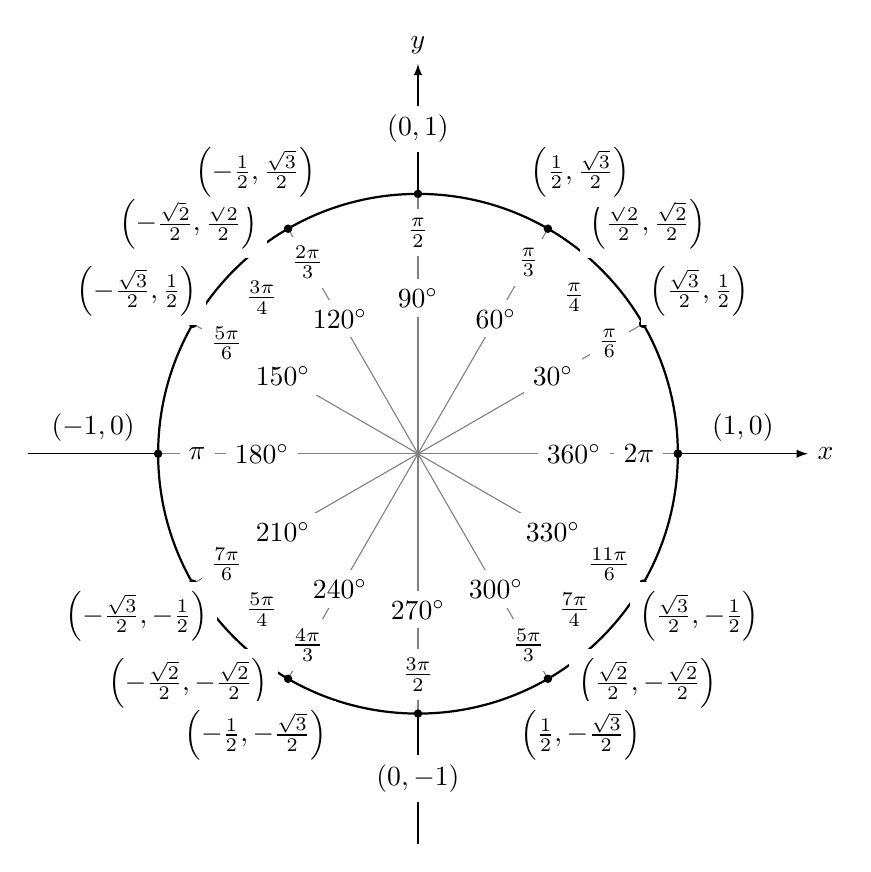
\begin{tikzpicture}[scale=3.3,cap=round,>=latex]
        % draw the coordinates
        \draw[->] (-1.5cm,0cm) -- (1.5cm,0cm) node[right,fill=white] {$x$};
        \draw[->] (0cm,-1.5cm) -- (0cm,1.5cm) node[above,fill=white] {$y$};

        % draw the unit circle
        \draw[thick] (0cm,0cm) circle(1cm);

        \foreach \x in {0,30,...,360} {
                % lines from center to point
                \draw[gray] (0cm,0cm) -- (\x:1cm);
                % dots at each point
                \filldraw[black] (\x:1cm) circle(0.4pt);
                % draw each angle in degrees
                \draw (\x:0.6cm) node[fill=white] {$\x^\circ$};
        }

        % draw each angle in radians
        \foreach \x/\xtext in {
            30/\frac{\pi}{6},
            45/\frac{\pi}{4},
            60/\frac{\pi}{3},
            90/\frac{\pi}{2},
            120/\frac{2\pi}{3},
            135/\frac{3\pi}{4},
            150/\frac{5\pi}{6},
            180/\pi,
            210/\frac{7\pi}{6},
            225/\frac{5\pi}{4},
            240/\frac{4\pi}{3},
            270/\frac{3\pi}{2},
            300/\frac{5\pi}{3},
            315/\frac{7\pi}{4},
            330/\frac{11\pi}{6},
            360/2\pi}
                \draw (\x:0.85cm) node[fill=white] {$\xtext$};

        \foreach \x/\xtext/\y in {
            % the coordinates for the first quadrant
            30/\frac{\sqrt{3}}{2}/\frac{1}{2},
            45/\frac{\sqrt{2}}{2}/\frac{\sqrt{2}}{2},
            60/\frac{1}{2}/\frac{\sqrt{3}}{2},
            % the coordinates for the second quadrant
            150/-\frac{\sqrt{3}}{2}/\frac{1}{2},
            135/-\frac{\sqrt{2}}{2}/\frac{\sqrt{2}}{2},
            120/-\frac{1}{2}/\frac{\sqrt{3}}{2},
            % the coordinates for the third quadrant
            210/-\frac{\sqrt{3}}{2}/-\frac{1}{2},
            225/-\frac{\sqrt{2}}{2}/-\frac{\sqrt{2}}{2},
            240/-\frac{1}{2}/-\frac{\sqrt{3}}{2},
            % the coordinates for the fourth quadrant
            330/\frac{\sqrt{3}}{2}/-\frac{1}{2},
            315/\frac{\sqrt{2}}{2}/-\frac{\sqrt{2}}{2},
            300/\frac{1}{2}/-\frac{\sqrt{3}}{2}}
                \draw (\x:1.25cm) node[fill=white] {$\left(\xtext,\y\right)$};

        % draw the horizontal and vertical coordinates
        % the placement is better this way
        \draw (-1.25cm,0cm) node[above=1pt] {$(-1,0)$}
              (1.25cm,0cm)  node[above=1pt] {$(1,0)$}
              (0cm,-1.25cm) node[fill=white] {$(0,-1)$}
              (0cm,1.25cm)  node[fill=white] {$(0,1)$};
    \end{tikzpicture}
}

% \definecolor{PaleVioletRed3}{RGB}{219,112,147} % PaleVioletRed
% \definecolor{PaleVioletRed3}{RGB}{255,102,255} % Pink

\newlength{\seplinewidth}
\newlength{\seplinesep}
\setlength{\seplinewidth}{1mm}
\setlength{\seplinesep}{2mm}
% \colorlet{sepline}{PaleVioletRed3}
\newcommand*{\sepline}{%
  \par
  \vspace{\dimexpr\seplinesep+.5\parskip}%
  \cleaders\vbox{%
    \begingroup % because of color
      \color{sepline}%
      \hrule width\linewidth height\seplinewidth
    \endgroup
  }\vskip\seplinewidth
  \vspace{\dimexpr\seplinesep-.5\parskip}%
}

% Define some colors
\definecolor{PaleVioletRed3}{RGB}{153,51,255} % Purple 
\definecolor{c_grey}{RGB}{247,247,247} % Grey 
\definecolor{c_grey2}{RGB}{213,213,213} % Grey 
\definecolor{c_note}{HTML}{000000} % Gold color for the note icon
\definecolor{theoremlightblue}{HTML}{F2F6FB}
\definecolor{theoremdarkblue}{HTML}{086FBD}
\definecolor{definitionlightgreen}{HTML}{F2F9F5}
\definecolor{definitiondarkgreen}{HTML}{129F57}
\definecolor{examplelightred}{HTML}{FFF5F6}
\definecolor{exampledarkred}{HTML}{FF3769}

% Global minted options
\setminted[]{breaklines, breakanywhere, autogobble, linenos=true, xleftmargin=20pt, mathescape}

% Begin minted code boxes
\tcbuselibrary{minted, skins}
\newtcblisting{cppcode}{
  arc=10pt,
  outer arc=10pt,
  listing only,
  minted style=xcode,
  minted language=cpp,
  minted options={linenos=true, breaklines=true},
  colback=c_grey,
  colframe=c_grey2,
  listing engine=minted,
  % other settings...
}

\newtcblisting{csscode}{
  arc=10pt,
  outer arc=10pt,
  listing only,
  minted style=xcode,
  minted language=css,
  minted options={linenos=true, breaklines=true},
  colback=c_grey,
  colframe=c_grey2,
  listing engine=minted,
  % other settings...
}

\newtcblisting{htmlcode}{
  arc=10pt,
  outer arc=10pt,
  listing only,
  minted style=xcode,
  minted language=html,
  minted options={linenos=true, breaklines=true},
  colback=c_grey,
  colframe=c_grey2,
  listing engine=minted,
  % other settings...
}

\newtcblisting{pythoncode}{
  arc=10pt,
  outer arc=10pt,
  listing only,
  minted style=xcode,
  minted language=python,
  minted options={linenos=true, breaklines=true},
  colback=c_grey,
  colframe=c_grey2,
  listing engine=minted,
  % other settings...
}

\newtcblisting{bashcode}{
  arc=10pt,
  outer arc=10pt,
  listing only,
  minted style=xcode,
  minted language=bash,
  minted options={linenos=true, breaklines=true},
  colback=c_grey,
  colframe=c_grey2,
  listing engine=minted,
  % other settings...
}

% End minted code boxes

% Color boxes
\newtcolorbox{notebox}{
  breakable,
  colback=c_grey,
  colframe=c_grey,
  boxrule=0pt,
  leftrule=5pt,
  colframe=c_grey2,
  arc=0pt,
  left=6pt,
  right=6pt,
  top=6pt,
  bottom=6pt,
  title=\faTired\ Note:, % Note title with icon
  coltitle=c_note, % Color of the title
  fonttitle=\bfseries, % Bold title font
  enhanced, % Enhanced mode for more features
  % overlay={%
  %   \node[anchor=north west, text=c_note] at (frame.north west) {\faTired}; % Note icon
  % }
}
\makeatother
\usepackage{thmtools}
\theoremstyle{definition}
\tcbuselibrary{theorems}
\declaretheoremstyle[
    headfont=\bfseries\sffamily\color{definitiondarkgreen!70!black}, bodyfont=\normalfont,
    mdframed={
            linewidth=2pt,
            rightline=false, topline=false, bottomline=false,
            linecolor=definitiondarkgreen, backgroundcolor=definitionlightgreen,
            nobreak=false
        }
]{thmgreenbox}

\declaretheoremstyle[
    headfont=\bfseries\sffamily\color{theoremdarkblue!70!black}, bodyfont=\normalfont,
    mdframed={
            linewidth=2pt,
            rightline=false, topline=false, bottomline=false,
            linecolor=theoremdarkblue, backgroundcolor=theoremlightblue,
            nobreak=false
        }
]{thmbluebox}

\declaretheoremstyle[
    headfont=\bfseries\sffamily\color{exampledarkred!70!black}, bodyfont=\normalfont,
    mdframed={
            linewidth=2pt,
            rightline=false, topline=false, bottomline=false,
            linecolor=exampledarkred, backgroundcolor=examplelightred,
            nobreak=false
        }
]{thmredbox}

\declaretheorem[style=thmgreenbox, name=Definition, numberwithin=section]{dfn}
\declaretheorem[style=thmbluebox, name=Theorem, numberwithin=section]{thrmm}
\declaretheorem[style=thmredbox, name=Example, numberwithin=section]{exm}

% Gray word box
\newtcbox{\emp}{nobeforeafter, colframe=gray, colback=lightgray, boxrule=0.5pt, arc=4pt, boxsep=0pt, left=2pt, right=2pt, top=2pt, bottom=2pt, tcbox raise base}


% \newtcbtheorem[number within=section]{thrmm}{Theorem}{
%   breakable,
%   colback=theoremlightgreen,
%   colframe=theoremlightgreen,
%   boxrule=0pt,
%   leftrule=3pt,
%   colframe=theoremdarkgreen,
%   arc=0pt,
%   left=6pt,
%   detach title,
% before upper = \tcbtitle\par\smallskip,
%   right=6pt,
%   top=0pt,
%   bottom=6pt,
%   % title=\faTired\ Note:, % Note title with icon
%   coltitle=0, % Color of the title
%   fonttitle=\bfseries, % Bold title font
%   enhanced, % Enhanced mode for more features
%   % overlay={%
%   %   \node[anchor=north west, text=c_note] at (frame.north west) {\faTired}; % Note icon
%   % }
% }{th}


% \newtcolorbox{notebox}{
%   breakable, % to allow page breaks
%   colback=c_grey, % background color of the box
%   colframe=c_grey, % frame color
%   boxrule=0pt, % frame thickness (set to 0pt to remove the frame)
%   leftrule=5pt, % thickness of the left rule
%   colframe=c_grey2, % color of the frame and left rule
%   arc=0pt, % remove rounding of the corners
%   left=6pt, % inner left margin
%   right=6pt, % inner right margin
%   top=6pt, % inner top margin
%   bottom=6pt % inner bottom margin
% }
%
% Purple mdframed box -- use: {mdframed}[style=purplebox]
\mdfdefinestyle{purplebox}{
  linewidth=2pt,       % thickness of the border
  linecolor=PaleVioletRed3,    % color of the border
  backgroundcolor=white, % background color of the box
  roundcorner=5pt,     % if you want rounded corners
  innertopmargin=\baselineskip, % space added at the top of the box
  skipabove=\baselineskip  % space added above the box
}
\mdfdefinestyle{codebox}{
    linewidth=1.5pt,
    linecolor=c_grey2,
    backgroundcolor=c_grey,
    roundcorner=5pt,
    leftmargin=20pt, % Adjust as needed
    innertopmargin=10pt, % Adjust as needed
}
%
% \mdfdefinestyle{codebox} {
%   linewidth=1.5pt,       % thickness of the border
%   linecolor=c_grey2,    % color of the border
%   backgroundcolor=c_grey, % background color of the box
%   roundcorner=5pt,     % if you want rounded corners
%   % innertopmargin=\baselineskip, % space added at the top of the box
%   % skipabove=\baselineskip  % space added above the box
% }

% \surroundwithmdframed{minted}

% \newcommand{\fa}{\ \forall\ }

% Some auxiliary defines 
\newcommand{\te}[1][]{\ \exists#1\ }

% Increases size of sections
\titleformat{\section}
  {\huge\bfseries} % Change \Huge to desired size
  {\thesection}{1em}{}

\titleformat{\subsection}
  {\large\bfseries} % Change \Huge to desired size
  {\thesubsection}{1em}{}

% Phantom sections
\newcommand{\unsect}[1]{
    \refstepcounter{section} % Increment section counter
    \addcontentsline{toc}{section}{\protect\numberline{\thesection}#1} % Add to TOC with number
    % \markboth{}{} % Remove header left
    %  \thispagestyle{empty} % Remove header right
   \markboth{\MakeUppercase{#1}}{}%
    \section*{#1} % Create unnumbered section
}

\newcommand{\beginch}[2] {
	\markboth{}{}
	 \vspace*{1.5in} % Add vertical space to push content down
	 \thispagestyle{empty}
     {\huge\bfseries Chapter #1} % Large, bold text
    \vspace*{.25in}
    \unsect{#2} % Call unsect command
    \bigbreak \noindent 
    \vspace*{.1in}
}
% Redefine \sectionmark
\renewcommand{\sectionmark}[1]{%
  \markboth{#1}{}%
}
% Page geometry
\geometry{
  left=1.5in,
  right=1.5in,
  top=1in,
  bottom=1in
}

